% Things that I have to cover:
% 1. Intro: Basics + History
% 2. Supervised Learning
% 3. Overfitting + Underfitting
% 4. Perceptron + Activation Functions
% 5. Loss Functions
% 6. Backpropagation
% 7. Optimization
% 8. Linear Regression
% 9. Neural Networks
% 10. Normalization
% 11. Gaussian Processes

In this chapter, we will discuss the machine learning techniques employed in this work. It does not aim to be a comprehensive guide to the subject, but rather a summary of the most important concepts and techniques so that the reader can understand the main ideas and the choices made in this work. One can refer to \cite{pml1Book} for a more detailed and comprehensive guide to the subject.

\section{Introduction}
In the recent years, machine learning, and particularly deep learning, has become a powerful tool in every scientific field. Some common examples include Large Language Models (LLMs) \cite{radford2019language,touvron2023llamaopenefficientfoundation}, synthetic image generation \cite{ho2020denoisingdiffusionprobabilisticmodels}, stellar astronomy \cite{ostdiek_b_cataloging_2020}, geoinformatics \cite{robin2022learningforecastvegetationgreenness}.

Let's begin by defining machine learning in a general way:

\begin{tcolorbox}[colback=red!5!white, colframe=red!75!black]
    An algorithm which is used to extract patterns and relationships from data, to make predictions, and to solve problems that are too complex to be solved by traditional methods.
\end{tcolorbox}

Since the development of advanced engineering tools and numerical programming, we have access to huge amount of data, and machine learning helps us to "learn" an intrinsic structure of it. 

This "learning" can be done in different ways, and we broadly classify them into three categories:
\begin{itemize}
    \item Supervised Learning
    \item Unsupervised Learning
    \item Reinforcement Learning
\end{itemize}

Since, our work focuses on the supervised learning, we will only discuss it in this chapter. However, later in this chapter, we will provide a brief overview of the other two types of learning.

\subsection{Supervised Learning}

\begin{figure}[t]
    \centering
    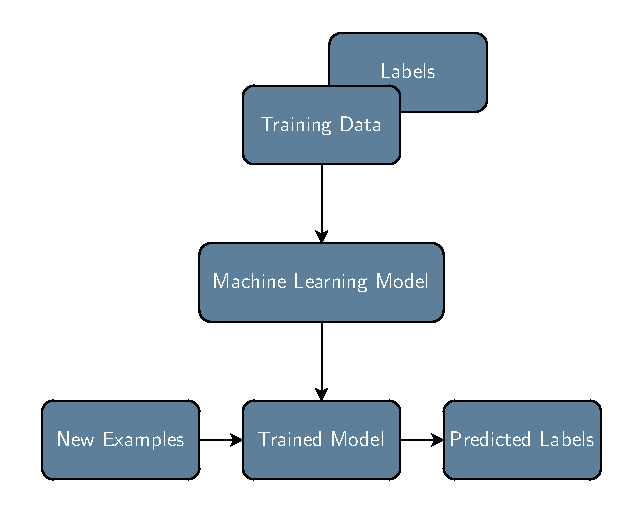
\includegraphics[scale=0.70]{chapter_03_ML/supervised_learn_pipeline.pdf} % [width=7cm, height=5cm]
    \caption{Supervised learning pipeline.}
    \label{fig:ml_pipeline_basic}
\end{figure}

The most common type of machine learning algorithm is the supervised learning. It is used when we have a dataset with labeled examples, and we want to learn a function $f$ that maps inputs $\textbf{x}$ to outputs $\textbf{y}$. Some examples of supervised learning problems include spam email detection, image classification, and speech recognition. The figure \ref{fig:ml_pipeline_basic} summarizes a typical supervised learning workflow, where the labeled training data is passed to a machine learning algorithm for fitting a predictive model that can make predictions on new, unlabeled data inputs.

Formally, the supervised learning problem can be written as:
\begin{equation}
    \label{eq:supervised_learning}
    \hat{\textbf{y}} = f(\textbf{x}; \theta).
\end{equation}

Here, both the input $\textbf{x}$ and output $\textbf{y}$ are vectors of a predetermined and fixed size. The model is just a mathematical equation with a fixed form. It represents a family of different relations between the input and the output. The model also contains \textit{parameters} $\theta$. The choice of parameters determines the particular relation between input and output.

When we talk about \textit{learning}, we mean that the model is able to find the \textbf{best parameters} $\theta$ that gives meaningful output for a given input. When we say meaningful, we mean that the model is able to generalize to new examples that it has not seen before. 

During the learning/training process, we learn the parameters using a set of training data of $N$ pairs of input and output $\{\textbf{x}_i, \textbf{y}_i\}$. We aim to modify these parameters such that map of each trainining input to its associated output as closely as possible. Therefore, in order to quantify the deviation between the predicted output and the target output, so that we can guide the training process, we define a \textit{loss function} $\mathcal{L}$. When we train the model, we aim to minimize this loss function:

\begin{equation}
    \theta^* = \operatorname*{argmin}_\theta \mathcal{L}(\mathcal{D}, \theta).
\end{equation}

There is a systematical way called \textit{optimization algorithm} to find the best parameters $\theta^*$ that help the model reach global or local minimum of the loss function. This will be discussed later in this chapter. 

Let's move on to discuss about the term dataset which comes up often in the context of machine learning.

\section{Dataset: Training, Validation, and Test Sets}

\begin{figure}[t]
    \centering
    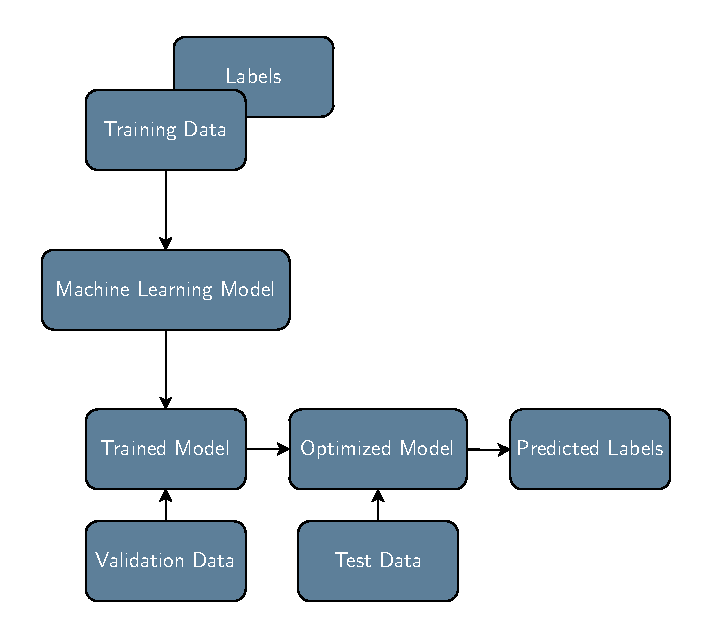
\includegraphics[scale=0.70]{chapter_03_ML/train_test_val_pipeline.pdf}
    \caption{Use of training, validation, and test sets.}
    \label{fig:dataset_split}
\end{figure}

The quality of the data and the amount of useful information that it contains are key factors that determine how well a machine learning algorithm can learn. Similarly, it is extremely necessary to split the collected data into different sets so that we can evaluate the performance of the model on unseen data. Based on the purpose, most of the machine learning pipelines are designed to split the data into three sets: training set, validation set, and test set.

\begin{itemize}
    \item Training set: This is the subset of data used to fit the model. Generally speaking, we randomly pick 70\% or 80\% of the data for training.
    \item Validation set: One of the most important sets which is often overlooked. Before the training process, we fix some of the parameters of the model called \textit{hyperparameters}. The validation set is used to tune these hyperparameters and plays a key role in diagnosing issues such as \textit{overfitting} and \textit{underfitting}. We split 15\% or 10\% of the data for validation.
    \item Test set: Finally, this is set of data which my model has not seen before. It serves as the final benchmark to assess the model’s performance, robustness, and generalization capability. Like the validation set, it typically comprises 10\% to 15\% of the total data. 
\end{itemize}

The role of each set can be clearly seen in the figure \ref{fig:dataset_split}.

In the next section, we will discuss about a point mentioned in the paragraph above: \textit{underfitting} and \textit{overfitting}.

\section{Headache: Overfitting and Underfitting}
In the world of machine learning, we rely on building a network of some fundamental building blocks (usually called \textit{neurons}) and achieving the right model complexity is an ongoing struggle. To give a brief idea about these concepts, we can say that \textit{overfitting} is when the model is "too complex" and it fits the training data too well, while \textit{underfitting} is when the model is "too simple" and it does not fit the training data well enough.

Let's take an example were we sample some data points from a 4th order polynomial function with some noise. Our goal is to develop a model that learns the underlying function (not exactly, but close enough). Now, while performing the training, we can have two different scenarios, one where model complexity is too low and it returns a quadratic function, and the other where model complexity is too high and it returns the 10th order polynomial function.

Overfitting corresponds to the case where the model output 10th order polynomial function, meaning it performs well on training data but does not generalize well to unseen data (test data). If a model suffers from overfitting, we also say that the model has a high variance, which can be caused by having too many parameters, leading to a model that is too complex given the underlying data.

Underfitting, on the other hand, corresponds to the case where the model output a linear function, meaning it performs poorly on both training and test data. If a model suffers from underfitting, we also say that the model has a high bias, which can be caused by having too few parameters, leading to a model that is too simple given the underlying data.

We can clearly see in the figure \ref{fig:overfitting_underfitting} the trade-off between model complexity and generalization, with overfitting resulting in excessive sensitivity to noise, and underfitting failing to capture the true underlying trend.

\begin{figure}[t]
    \centering
    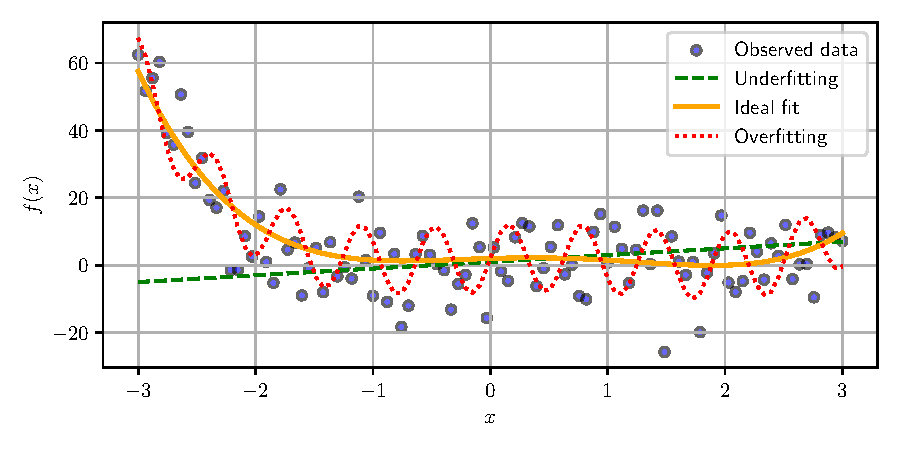
\includegraphics[scale=0.70]{chapter_03_ML/over_under_fit.pdf}
    \caption{Illustration of model underfitting, ideal fitting, and overfitting on noisy data generated from a 4th-order polynomial function. The data points (blue scatter) are sampled from the function $0.5x^4 - x^3 - x^2 + x + 2$ with some noise $\mathcal{N}(0, 10)$. The orange curve represents an underfit model (linear regression), the green curve shows the ideal 4th-order polynomial fit, and the red curve illustrates an overfit model, where a higher-degree polynomial captures the noise.}
    \label{fig:overfitting_underfitting}
\end{figure}

I want to make one thing clear at this point. There are certain keywords which have not been clearly defined in our discussion above. However, we will follow up on them in the upcoming sections. For now, let's move on to the next section where we will discuss about the heart of the machine learning model: \textit{neural networks}.

\section{Neural Networks}

The core idea of modern machine learning or deep learning lies in the idea of building effective and problem-specific neural networks. Let's take a look at what we mean by it and what is it's origin.

\subsection{Building Blocks: Perceptrons}

The origins of neural networks (or artificial neural networks) can be traced to the early 20th century, inspired by the biological neural networks that underpin cognitive functions in living organisms. This early work lead to the development of the perceptron, which is a simple model of a neuron (artificial neuron). This forms the basis of the modern neural networks where we have multiple layers of perceptrons.

A single perceptron is a simple model that takes multiple inputs, $\textbf{x} \in \mathbb{R}^n$, and produces a single scalar output, $y$. The output is a weighted sum of the inputs, plus a bias term is passed through an \textit{activation function}, $\sigma: \mathbb{R} \rightarrow \mathbb{R}$.

\begin{equation}
    y = \sigma \left( \textbf{w}^{\top} \textbf{x} + b \right)
    \label{eq:perceptron}
\end{equation}

where, $\textbf{w} \in \mathbb{R}^n$ is the weight vector and $b \in \mathbb{R}$ is the bias term.

\subsection{Multi-layer Perceptrons}


When we have multiple perceptrons, we can stack them up to form what we call a \textit{neural network}. The output of the first layer is the input of the second layer, and so on. This way, we can build a deep neural network. The layers between the input and output layers are called \textit{hidden layers}. We start with inputs $\textbf{x} \in \mathbb{R}^n$ and we have $L$ hidden layers. The output of the $l$-th hidden layer is given by:

\begin{equation}
    \textbf{h}_l = \sigma \left( \textbf{W}_l \textbf{h}_{l-1} + \textbf{b}_l \right)
    \label{eq:hidden_layer}
\end{equation}

where, $\textbf{W}_l \in \mathbb{R}^{n \times n_{l-1}}$ is the weight matrix and $\textbf{b}_l \in \mathbb{R}^{n_l}$ is the bias vector. It is these \textit{weights} and \textit{biases} which are the \textit{parameters} tuned during the training process.

As we see in the equation \ref{eq:perceptron} and \ref{eq:hidden_layer}, we have an entity called the activation function $\sigma$. It is this function which introduces non-linearity to the model. One can make multiple choices for the activation functions which mainly depends on the problem at hand. We will highlight some of them in the next section. 

\begin{figure}[t]
    \centering
    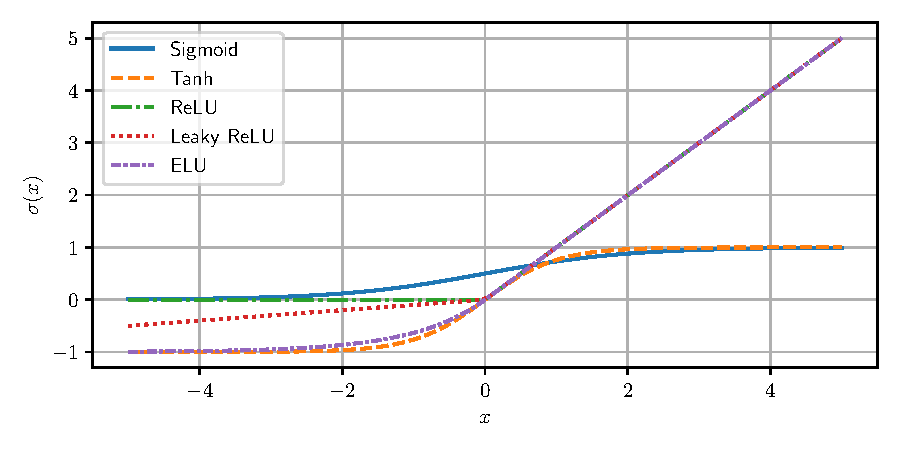
\includegraphics[scale=0.70]{chapter_03_ML/activations_func.pdf}
    \caption{Activation functions.}
    \label{fig:activation_functions}
\end{figure}

\subsection{Activation Functions}

A stack of linear layers is equivalent to a single linear layer where we multliply together all the weight matrices. To get more expressive power we can transform each layer by passing it elementwise (pointwise) through a nonlinear function called an activation function. In figure \ref{fig:activation_functions} and table \ref{tab:activation_functions}, we have highlighted some of the most common activation functions.

Mathematically, a suitable activation function is typically required to be non-linear and differentiable to allow effective learning through gradient-based optimization methods like \textit{backpropagation}. Additional desirable properties include boundedness (to prevent uncontrolled output growth), monotonicity (to aid convergence), and computational efficiency (to ensure scalability).

Just like previous sections, there are a few keywords which have not been defined in proper manner. I just want to make sure that reader is aware that they will be discussed in the upcoming sections.

\begin{table}[t]
    \centering
    \caption{Common Activation Functions in Neural Networks}
    \renewcommand{\arraystretch}{1.5} % Increases row height
    \begin{tabular}{|>{\centering\arraybackslash}m{3.5cm}|>{\centering\arraybackslash}m{5.5cm}|>{\centering\arraybackslash}m{5.5cm}|}
    \hline
    \textbf{Activation Function} & \textbf{Expression} & \textbf{Key Properties} \\
    \hline
    Sigmoid & 
    $\displaystyle \sigma(x) = \frac{1}{1 + e^{-x}}$ & 
    Bounded, smooth, vanishing gradients \\
    \hline
    Tanh & 
    $\displaystyle \tanh(x) = \frac{e^x - e^{-x}}{e^x + e^{-x}}$ & 
    Zero-centered, smooth, vanishing gradients \\
    \hline
    ReLU & 
    $\displaystyle \text{ReLU}(x) = \max(0, x)$ & 
    Sparse activations, fast computation, non-saturating \\
    \hline
    Leaky ReLU & 
    $\displaystyle \text{LeakyReLU}(x) = \begin{cases}
    x, & x > 0 \\
    \alpha x, & x \leq 0
    \end{cases}$ & 
    Avoids dead neurons, small negative slope \\
    \hline
    ELU & 
    $\displaystyle \text{ELU}(x) = \begin{cases}
    x, & x > 0 \\
    \alpha(e^x - 1), & x \leq 0
    \end{cases}$ & 
    Smooth, avoids vanishing gradient for $x < 0$ \\
    \hline
    \end{tabular}
    \label{tab:activation_functions}
\end{table}

\subsection{Loss Functions}


    














